\section{Durchführung}
\label{sec:Durchführung}

\subsection{Vermessung der Acrylzylinder}
Als erstes wird ein Acrylzylinder mit 
einer \SI{2}{\mega\hertz}-Sonde auf einer Schicht aus bidestiliertem 
Wassser gekoppelt. Damit wird ein A-Scan mittels 
Impuls-Echo-Verfahren durchgeführt. Für die ersten beiden 
Pulse werden die Laufzeit und Amplitude 
gemessen. 
Die Länge des Zylinders wird gemessen.
Diese Messung wird mit vier weiteren Acrylzylinder wiederholt.
Die Zylinder sind in Abb. \ref{fig:zylinder} zu sehen.
\begin{figure}
    \centering
    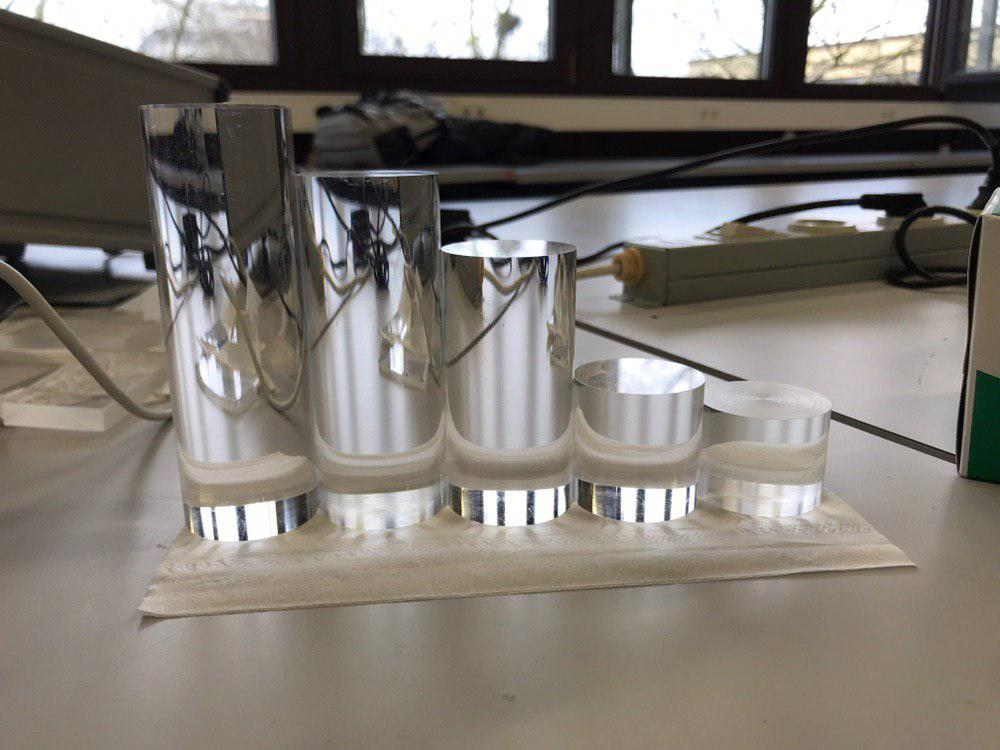
\includegraphics[width=12cm, height=8cm]{build/BildZylinder.jpg}
    \caption{Die verwendeten Acrylzylinder.}
    \label{fig:zylinder}
\end{figure}

\subsection{Bestimmung der Dämpfung mittels Impuls-Echo-Verfahren}
Aus den vorherigen Messungen wird für alle fünf Acrylzylinder
durch die Amplituden der materialspezifische Schwächungskoeffizient bestimmt.

\subsection{Bestimmung der Schallgeschwindigkeit mittels Durchschallungs-Verfahren}
Die Acrylzylinder werden in die Halterung gespannt und an 
beiden Seiten wird jeweils eine Sonde mit Koppelgel gekoppelt. 
Mit einem A-Scan wird die Laufzeit bestimmt, indem die Zeiten
der ersten beiden Amplituden gemessen werden. Die Messung wird für alle 
Zylinder wiederholt.
%"Zeiten der Amplituden" - ist das richtig formuliert?

\subsection{Bestimmung der Schallgeschwindigkeit mittels Impuls-Echo-Verfahren}
Die Acrylzylinder werden erneut mit dem Impuls-Echo-Verfahren
und einem A-Scan gemessen. Die Zeitpunkte der reflektierten Pulse
werden aufgenommen.

\subsection{Biometrische Untersuchung eines Augenmodells}
Die \SI{2}{\mega\hertz}-Sonde wird mit Koppelgel auf die
Hornhaut des Augenmodells, das in Abb. \ref{fig:bild_augenmodell} zu sehen ist, gesetzt. Mit einem A-Scan werden die
Echos an den Grenzflächen der Iris und der Retina (siehe Abb. \ref{fig:augenmodell}) aufgenommen.
Aus den Zeitpunkten können die Abmessungen des Auges bestimmt 
werden.
\begin{figure}
    \centering
    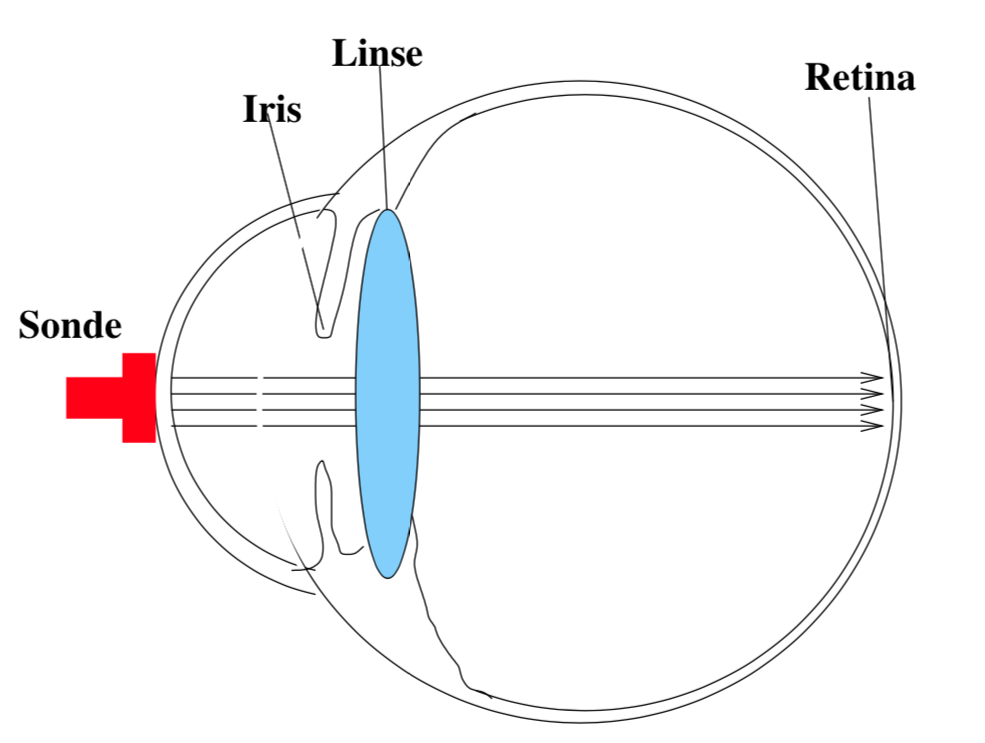
\includegraphics[width=12cm, height=8cm]{build/Augenmodell.png}
    \caption{Das Modell eines Auges. \cite{US1}}
    \label{fig:augenmodell}
\end{figure}
\begin{figure}
    \centering
    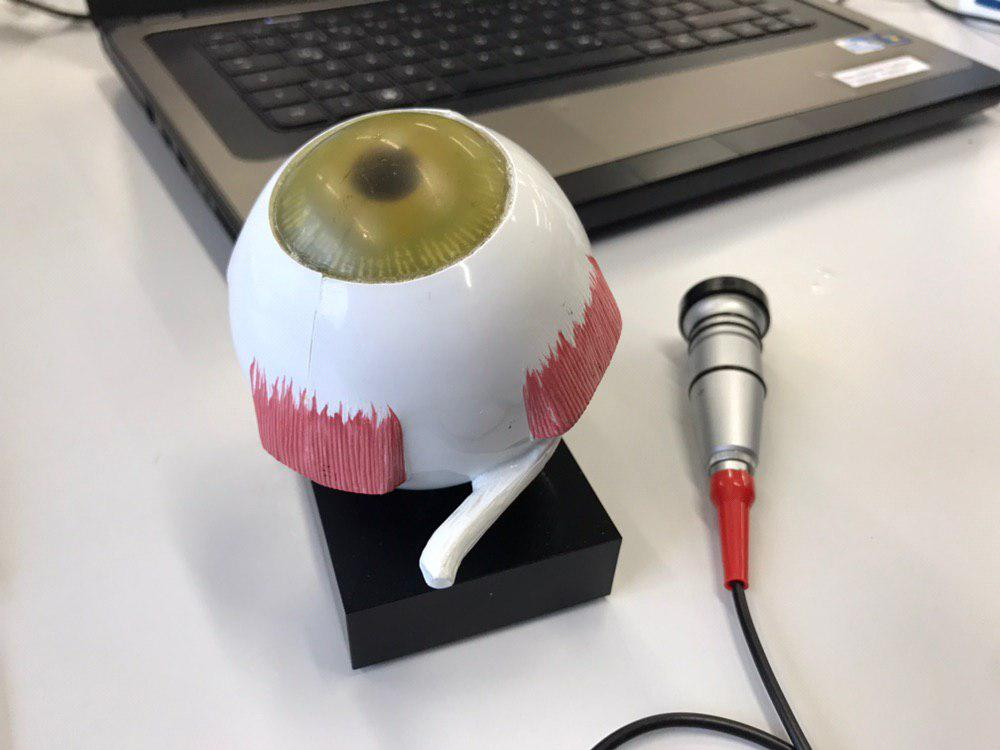
\includegraphics[width=12cm, height=8cm]{build/BildAuge.jpg}
    \caption{Foto des untersuchten Augenmodells.}
    \label{fig:bild_augenmodell}
\end{figure}